% https://tex.stackexchange.com/questions/538319/drawing-complicated-geometry-figures-in-tikz

\documentclass[tikz,border=3mm]{standalone}
\usetikzlibrary{angles,calc,intersections}
\begin{document}
  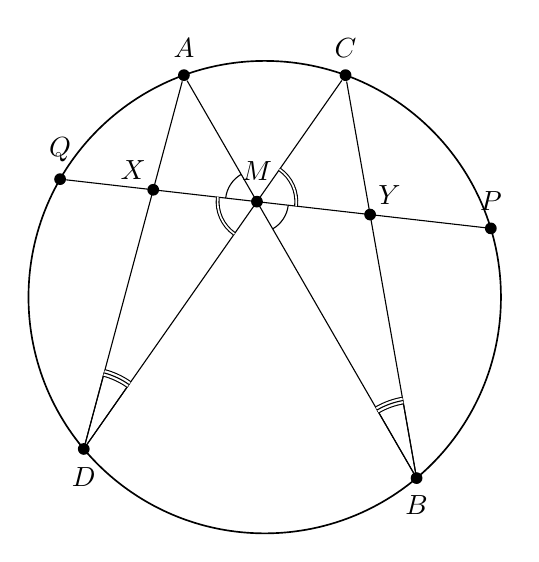
\begin{tikzpicture}[declare function={R=3;},
    dot/.style={circle,fill,inner sep=1.5pt},
    tarc/.style={draw,double distance=2pt,angle radius=10mm,
    pic actions/.append code=\tikzset{postaction={draw}}},
    sarc/.style={draw,angle radius=4mm},
    darc/.style={draw,double,angle radius=5mm},
   ]
   \begin{scope}[nodes={dot}]
     \draw[name path=circ,semithick]   (0,0) coordinate (O) circle[radius=R];  
     \path (110:R) node[label=above:$A$] (A){}
       (-50:R) node[label=below:$B$] (B){}     
       (70:R) node[label=above:$C$] (C){}
       (220:R) node[label=below:$D$] (D){}
       (intersection of A--B and C--D) node[label=above:$M$] (M){}
       (A) -- (D) node[pos=0.3,label=above left:$X$](X){};
     \path[overlay,name path=line] let \p1=($(M)-(X)$),\n1={atan2(\y1,\x1)} in
       ($(M)+(\n1:10)$) --  ($(M)+(\n1+180:10)$);
     \path[name intersections={of=circ and line,by={P,Q}},nodes={dot}]
       (P) node[label=above:$P$]{} (Q) node[label=above:$Q$]{};
     \draw[fill=none] (A) -- (D) -- (C) -- (B) -- (A) (P) -- (Q) 
       (intersection of P--Q and C--B) node[dot,label=above right:$Y$] (Y){};
   \end{scope}        
   \path pic[tarc]{angle={C--D--A}}
     pic[tarc]{angle={C--B--A}}
     pic[darc]{angle={Q--M--D}}
     pic[darc]{angle={P--M--C}}
     pic[sarc]{angle={B--M--P}}
     pic[sarc]{angle={A--M--Q}};
\end{tikzpicture}
\end{document}